\documentclass[10pt]{article}
% Anonymous submission format of TMLR. Use [preprint] for an arXiv version.
\usepackage{tmlr}
%%%%% NEW MATH DEFINITIONS %%%%%

\usepackage{amsmath,amsfonts,bm}

% Mark sections of captions for referring to divisions of figures
\newcommand{\figleft}{{\em (Left)}}
\newcommand{\figcenter}{{\em (Center)}}
\newcommand{\figright}{{\em (Right)}}
\newcommand{\figtop}{{\em (Top)}}
\newcommand{\figbottom}{{\em (Bottom)}}
\newcommand{\captiona}{{\em (a)}}
\newcommand{\captionb}{{\em (b)}}
\newcommand{\captionc}{{\em (c)}}
\newcommand{\captiond}{{\em (d)}}

% Highlight a newly defined term
\newcommand{\newterm}[1]{{\bf #1}}


% Figure reference, lower-case.
\def\figref#1{figure~\ref{#1}}
% Figure reference, capital. For start of sentence
\def\Figref#1{Figure~\ref{#1}}
\def\twofigref#1#2{figures \ref{#1} and \ref{#2}}
\def\quadfigref#1#2#3#4{figures \ref{#1}, \ref{#2}, \ref{#3} and \ref{#4}}
% Section reference, lower-case.
\def\secref#1{section~\ref{#1}}
% Section reference, capital.
\def\Secref#1{Section~\ref{#1}}
% Reference to two sections.
\def\twosecrefs#1#2{sections \ref{#1} and \ref{#2}}
% Reference to three sections.
\def\secrefs#1#2#3{sections \ref{#1}, \ref{#2} and \ref{#3}}
% Reference to an equation, lower-case.
\def\eqref#1{equation~\ref{#1}}
% Reference to an equation, upper case
\def\Eqref#1{Equation~\ref{#1}}
% A raw reference to an equation---avoid using if possible
\def\plaineqref#1{\ref{#1}}
% Reference to a chapter, lower-case.
\def\chapref#1{chapter~\ref{#1}}
% Reference to an equation, upper case.
\def\Chapref#1{Chapter~\ref{#1}}
% Reference to a range of chapters
\def\rangechapref#1#2{chapters\ref{#1}--\ref{#2}}
% Reference to an algorithm, lower-case.
\def\algref#1{algorithm~\ref{#1}}
% Reference to an algorithm, upper case.
\def\Algref#1{Algorithm~\ref{#1}}
\def\twoalgref#1#2{algorithms \ref{#1} and \ref{#2}}
\def\Twoalgref#1#2{Algorithms \ref{#1} and \ref{#2}}
% Reference to a part, lower case
\def\partref#1{part~\ref{#1}}
% Reference to a part, upper case
\def\Partref#1{Part~\ref{#1}}
\def\twopartref#1#2{parts \ref{#1} and \ref{#2}}

\def\ceil#1{\lceil #1 \rceil}
\def\floor#1{\lfloor #1 \rfloor}
\def\1{\bm{1}}
\newcommand{\train}{\mathcal{D}}
\newcommand{\valid}{\mathcal{D_{\mathrm{valid}}}}
\newcommand{\test}{\mathcal{D_{\mathrm{test}}}}

\def\eps{{\epsilon}}


% Random variables
\def\reta{{\textnormal{$\eta$}}}
\def\ra{{\textnormal{a}}}
\def\rb{{\textnormal{b}}}
\def\rc{{\textnormal{c}}}
\def\rd{{\textnormal{d}}}
\def\re{{\textnormal{e}}}
\def\rf{{\textnormal{f}}}
\def\rg{{\textnormal{g}}}
\def\rh{{\textnormal{h}}}
\def\ri{{\textnormal{i}}}
\def\rj{{\textnormal{j}}}
\def\rk{{\textnormal{k}}}
\def\rl{{\textnormal{l}}}
% rm is already a command, just don't name any random variables m
\def\rn{{\textnormal{n}}}
\def\ro{{\textnormal{o}}}
\def\rp{{\textnormal{p}}}
\def\rq{{\textnormal{q}}}
\def\rr{{\textnormal{r}}}
\def\rs{{\textnormal{s}}}
\def\rt{{\textnormal{t}}}
\def\ru{{\textnormal{u}}}
\def\rv{{\textnormal{v}}}
\def\rw{{\textnormal{w}}}
\def\rx{{\textnormal{x}}}
\def\ry{{\textnormal{y}}}
\def\rz{{\textnormal{z}}}

% Random vectors
\def\rvepsilon{{\mathbf{\epsilon}}}
\def\rvtheta{{\mathbf{\theta}}}
\def\rva{{\mathbf{a}}}
\def\rvb{{\mathbf{b}}}
\def\rvc{{\mathbf{c}}}
\def\rvd{{\mathbf{d}}}
\def\rve{{\mathbf{e}}}
\def\rvf{{\mathbf{f}}}
\def\rvg{{\mathbf{g}}}
\def\rvh{{\mathbf{h}}}
\def\rvu{{\mathbf{i}}}
\def\rvj{{\mathbf{j}}}
\def\rvk{{\mathbf{k}}}
\def\rvl{{\mathbf{l}}}
\def\rvm{{\mathbf{m}}}
\def\rvn{{\mathbf{n}}}
\def\rvo{{\mathbf{o}}}
\def\rvp{{\mathbf{p}}}
\def\rvq{{\mathbf{q}}}
\def\rvr{{\mathbf{r}}}
\def\rvs{{\mathbf{s}}}
\def\rvt{{\mathbf{t}}}
\def\rvu{{\mathbf{u}}}
\def\rvv{{\mathbf{v}}}
\def\rvw{{\mathbf{w}}}
\def\rvx{{\mathbf{x}}}
\def\rvy{{\mathbf{y}}}
\def\rvz{{\mathbf{z}}}

% Elements of random vectors
\def\erva{{\textnormal{a}}}
\def\ervb{{\textnormal{b}}}
\def\ervc{{\textnormal{c}}}
\def\ervd{{\textnormal{d}}}
\def\erve{{\textnormal{e}}}
\def\ervf{{\textnormal{f}}}
\def\ervg{{\textnormal{g}}}
\def\ervh{{\textnormal{h}}}
\def\ervi{{\textnormal{i}}}
\def\ervj{{\textnormal{j}}}
\def\ervk{{\textnormal{k}}}
\def\ervl{{\textnormal{l}}}
\def\ervm{{\textnormal{m}}}
\def\ervn{{\textnormal{n}}}
\def\ervo{{\textnormal{o}}}
\def\ervp{{\textnormal{p}}}
\def\ervq{{\textnormal{q}}}
\def\ervr{{\textnormal{r}}}
\def\ervs{{\textnormal{s}}}
\def\ervt{{\textnormal{t}}}
\def\ervu{{\textnormal{u}}}
\def\ervv{{\textnormal{v}}}
\def\ervw{{\textnormal{w}}}
\def\ervx{{\textnormal{x}}}
\def\ervy{{\textnormal{y}}}
\def\ervz{{\textnormal{z}}}

% Random matrices
\def\rmA{{\mathbf{A}}}
\def\rmB{{\mathbf{B}}}
\def\rmC{{\mathbf{C}}}
\def\rmD{{\mathbf{D}}}
\def\rmE{{\mathbf{E}}}
\def\rmF{{\mathbf{F}}}
\def\rmG{{\mathbf{G}}}
\def\rmH{{\mathbf{H}}}
\def\rmI{{\mathbf{I}}}
\def\rmJ{{\mathbf{J}}}
\def\rmK{{\mathbf{K}}}
\def\rmL{{\mathbf{L}}}
\def\rmM{{\mathbf{M}}}
\def\rmN{{\mathbf{N}}}
\def\rmO{{\mathbf{O}}}
\def\rmP{{\mathbf{P}}}
\def\rmQ{{\mathbf{Q}}}
\def\rmR{{\mathbf{R}}}
\def\rmS{{\mathbf{S}}}
\def\rmT{{\mathbf{T}}}
\def\rmU{{\mathbf{U}}}
\def\rmV{{\mathbf{V}}}
\def\rmW{{\mathbf{W}}}
\def\rmX{{\mathbf{X}}}
\def\rmY{{\mathbf{Y}}}
\def\rmZ{{\mathbf{Z}}}

% Elements of random matrices
\def\ermA{{\textnormal{A}}}
\def\ermB{{\textnormal{B}}}
\def\ermC{{\textnormal{C}}}
\def\ermD{{\textnormal{D}}}
\def\ermE{{\textnormal{E}}}
\def\ermF{{\textnormal{F}}}
\def\ermG{{\textnormal{G}}}
\def\ermH{{\textnormal{H}}}
\def\ermI{{\textnormal{I}}}
\def\ermJ{{\textnormal{J}}}
\def\ermK{{\textnormal{K}}}
\def\ermL{{\textnormal{L}}}
\def\ermM{{\textnormal{M}}}
\def\ermN{{\textnormal{N}}}
\def\ermO{{\textnormal{O}}}
\def\ermP{{\textnormal{P}}}
\def\ermQ{{\textnormal{Q}}}
\def\ermR{{\textnormal{R}}}
\def\ermS{{\textnormal{S}}}
\def\ermT{{\textnormal{T}}}
\def\ermU{{\textnormal{U}}}
\def\ermV{{\textnormal{V}}}
\def\ermW{{\textnormal{W}}}
\def\ermX{{\textnormal{X}}}
\def\ermY{{\textnormal{Y}}}
\def\ermZ{{\textnormal{Z}}}

% Vectors
\def\vzero{{\bm{0}}}
\def\vone{{\bm{1}}}
\def\vmu{{\bm{\mu}}}
\def\vtheta{{\bm{\theta}}}
\def\va{{\bm{a}}}
\def\vb{{\bm{b}}}
\def\vc{{\bm{c}}}
\def\vd{{\bm{d}}}
\def\ve{{\bm{e}}}
\def\vf{{\bm{f}}}
\def\vg{{\bm{g}}}
\def\vh{{\bm{h}}}
\def\vi{{\bm{i}}}
\def\vj{{\bm{j}}}
\def\vk{{\bm{k}}}
\def\vl{{\bm{l}}}
\def\vm{{\bm{m}}}
\def\vn{{\bm{n}}}
\def\vo{{\bm{o}}}
\def\vp{{\bm{p}}}
\def\vq{{\bm{q}}}
\def\vr{{\bm{r}}}
\def\vs{{\bm{s}}}
\def\vt{{\bm{t}}}
\def\vu{{\bm{u}}}
\def\vv{{\bm{v}}}
\def\vw{{\bm{w}}}
\def\vx{{\bm{x}}}
\def\vy{{\bm{y}}}
\def\vz{{\bm{z}}}

% Elements of vectors
\def\evalpha{{\alpha}}
\def\evbeta{{\beta}}
\def\evepsilon{{\epsilon}}
\def\evlambda{{\lambda}}
\def\evomega{{\omega}}
\def\evmu{{\mu}}
\def\evpsi{{\psi}}
\def\evsigma{{\sigma}}
\def\evtheta{{\theta}}
\def\eva{{a}}
\def\evb{{b}}
\def\evc{{c}}
\def\evd{{d}}
\def\eve{{e}}
\def\evf{{f}}
\def\evg{{g}}
\def\evh{{h}}
\def\evi{{i}}
\def\evj{{j}}
\def\evk{{k}}
\def\evl{{l}}
\def\evm{{m}}
\def\evn{{n}}
\def\evo{{o}}
\def\evp{{p}}
\def\evq{{q}}
\def\evr{{r}}
\def\evs{{s}}
\def\evt{{t}}
\def\evu{{u}}
\def\evv{{v}}
\def\evw{{w}}
\def\evx{{x}}
\def\evy{{y}}
\def\evz{{z}}

% Matrix
\def\mA{{\bm{A}}}
\def\mB{{\bm{B}}}
\def\mC{{\bm{C}}}
\def\mD{{\bm{D}}}
\def\mE{{\bm{E}}}
\def\mF{{\bm{F}}}
\def\mG{{\bm{G}}}
\def\mH{{\bm{H}}}
\def\mI{{\bm{I}}}
\def\mJ{{\bm{J}}}
\def\mK{{\bm{K}}}
\def\mL{{\bm{L}}}
\def\mM{{\bm{M}}}
\def\mN{{\bm{N}}}
\def\mO{{\bm{O}}}
\def\mP{{\bm{P}}}
\def\mQ{{\bm{Q}}}
\def\mR{{\bm{R}}}
\def\mS{{\bm{S}}}
\def\mT{{\bm{T}}}
\def\mU{{\bm{U}}}
\def\mV{{\bm{V}}}
\def\mW{{\bm{W}}}
\def\mX{{\bm{X}}}
\def\mY{{\bm{Y}}}
\def\mZ{{\bm{Z}}}
\def\mBeta{{\bm{\beta}}}
\def\mPhi{{\bm{\Phi}}}
\def\mLambda{{\bm{\Lambda}}}
\def\mSigma{{\bm{\Sigma}}}

% Tensor
\DeclareMathAlphabet{\mathsfit}{\encodingdefault}{\sfdefault}{m}{sl}
\SetMathAlphabet{\mathsfit}{bold}{\encodingdefault}{\sfdefault}{bx}{n}
\newcommand{\tens}[1]{\bm{\mathsfit{#1}}}
\def\tA{{\tens{A}}}
\def\tB{{\tens{B}}}
\def\tC{{\tens{C}}}
\def\tD{{\tens{D}}}
\def\tE{{\tens{E}}}
\def\tF{{\tens{F}}}
\def\tG{{\tens{G}}}
\def\tH{{\tens{H}}}
\def\tI{{\tens{I}}}
\def\tJ{{\tens{J}}}
\def\tK{{\tens{K}}}
\def\tL{{\tens{L}}}
\def\tM{{\tens{M}}}
\def\tN{{\tens{N}}}
\def\tO{{\tens{O}}}
\def\tP{{\tens{P}}}
\def\tQ{{\tens{Q}}}
\def\tR{{\tens{R}}}
\def\tS{{\tens{S}}}
\def\tT{{\tens{T}}}
\def\tU{{\tens{U}}}
\def\tV{{\tens{V}}}
\def\tW{{\tens{W}}}
\def\tX{{\tens{X}}}
\def\tY{{\tens{Y}}}
\def\tZ{{\tens{Z}}}


% Graph
\def\gA{{\mathcal{A}}}
\def\gB{{\mathcal{B}}}
\def\gC{{\mathcal{C}}}
\def\gD{{\mathcal{D}}}
\def\gE{{\mathcal{E}}}
\def\gF{{\mathcal{F}}}
\def\gG{{\mathcal{G}}}
\def\gH{{\mathcal{H}}}
\def\gI{{\mathcal{I}}}
\def\gJ{{\mathcal{J}}}
\def\gK{{\mathcal{K}}}
\def\gL{{\mathcal{L}}}
\def\gM{{\mathcal{M}}}
\def\gN{{\mathcal{N}}}
\def\gO{{\mathcal{O}}}
\def\gP{{\mathcal{P}}}
\def\gQ{{\mathcal{Q}}}
\def\gR{{\mathcal{R}}}
\def\gS{{\mathcal{S}}}
\def\gT{{\mathcal{T}}}
\def\gU{{\mathcal{U}}}
\def\gV{{\mathcal{V}}}
\def\gW{{\mathcal{W}}}
\def\gX{{\mathcal{X}}}
\def\gY{{\mathcal{Y}}}
\def\gZ{{\mathcal{Z}}}

% Sets
\def\sA{{\mathbb{A}}}
\def\sB{{\mathbb{B}}}
\def\sC{{\mathbb{C}}}
\def\sD{{\mathbb{D}}}
% Don't use a set called E, because this would be the same as our symbol
% for expectation.
\def\sF{{\mathbb{F}}}
\def\sG{{\mathbb{G}}}
\def\sH{{\mathbb{H}}}
\def\sI{{\mathbb{I}}}
\def\sJ{{\mathbb{J}}}
\def\sK{{\mathbb{K}}}
\def\sL{{\mathbb{L}}}
\def\sM{{\mathbb{M}}}
\def\sN{{\mathbb{N}}}
\def\sO{{\mathbb{O}}}
\def\sP{{\mathbb{P}}}
\def\sQ{{\mathbb{Q}}}
\def\sR{{\mathbb{R}}}
\def\sS{{\mathbb{S}}}
\def\sT{{\mathbb{T}}}
\def\sU{{\mathbb{U}}}
\def\sV{{\mathbb{V}}}
\def\sW{{\mathbb{W}}}
\def\sX{{\mathbb{X}}}
\def\sY{{\mathbb{Y}}}
\def\sZ{{\mathbb{Z}}}

% Entries of a matrix
\def\emLambda{{\Lambda}}
\def\emA{{A}}
\def\emB{{B}}
\def\emC{{C}}
\def\emD{{D}}
\def\emE{{E}}
\def\emF{{F}}
\def\emG{{G}}
\def\emH{{H}}
\def\emI{{I}}
\def\emJ{{J}}
\def\emK{{K}}
\def\emL{{L}}
\def\emM{{M}}
\def\emN{{N}}
\def\emO{{O}}
\def\emP{{P}}
\def\emQ{{Q}}
\def\emR{{R}}
\def\emS{{S}}
\def\emT{{T}}
\def\emU{{U}}
\def\emV{{V}}
\def\emW{{W}}
\def\emX{{X}}
\def\emY{{Y}}
\def\emZ{{Z}}
\def\emSigma{{\Sigma}}

% entries of a tensor
% Same font as tensor, without \bm wrapper
\newcommand{\etens}[1]{\mathsfit{#1}}
\def\etLambda{{\etens{\Lambda}}}
\def\etA{{\etens{A}}}
\def\etB{{\etens{B}}}
\def\etC{{\etens{C}}}
\def\etD{{\etens{D}}}
\def\etE{{\etens{E}}}
\def\etF{{\etens{F}}}
\def\etG{{\etens{G}}}
\def\etH{{\etens{H}}}
\def\etI{{\etens{I}}}
\def\etJ{{\etens{J}}}
\def\etK{{\etens{K}}}
\def\etL{{\etens{L}}}
\def\etM{{\etens{M}}}
\def\etN{{\etens{N}}}
\def\etO{{\etens{O}}}
\def\etP{{\etens{P}}}
\def\etQ{{\etens{Q}}}
\def\etR{{\etens{R}}}
\def\etS{{\etens{S}}}
\def\etT{{\etens{T}}}
\def\etU{{\etens{U}}}
\def\etV{{\etens{V}}}
\def\etW{{\etens{W}}}
\def\etX{{\etens{X}}}
\def\etY{{\etens{Y}}}
\def\etZ{{\etens{Z}}}

% The true underlying data generating distribution
\newcommand{\pdata}{p_{\rm{data}}}
% The empirical distribution defined by the training set
\newcommand{\ptrain}{\hat{p}_{\rm{data}}}
\newcommand{\Ptrain}{\hat{P}_{\rm{data}}}
% The model distribution
\newcommand{\pmodel}{p_{\rm{model}}}
\newcommand{\Pmodel}{P_{\rm{model}}}
\newcommand{\ptildemodel}{\tilde{p}_{\rm{model}}}
% Stochastic autoencoder distributions
\newcommand{\pencode}{p_{\rm{encoder}}}
\newcommand{\pdecode}{p_{\rm{decoder}}}
\newcommand{\precons}{p_{\rm{reconstruct}}}

\newcommand{\laplace}{\mathrm{Laplace}} % Laplace distribution

\newcommand{\E}{\mathbb{E}}
\newcommand{\Ls}{\mathcal{L}}
\newcommand{\R}{\mathbb{R}}
\newcommand{\emp}{\tilde{p}}
\newcommand{\lr}{\alpha}
\newcommand{\reg}{\lambda}
\newcommand{\rect}{\mathrm{rectifier}}
\newcommand{\softmax}{\mathrm{softmax}}
\newcommand{\sigmoid}{\sigma}
\newcommand{\softplus}{\zeta}
\newcommand{\KL}{D_{\mathrm{KL}}}
\newcommand{\Var}{\mathrm{Var}}
\newcommand{\standarderror}{\mathrm{SE}}
\newcommand{\Cov}{\mathrm{Cov}}
% Wolfram Mathworld says $L^2$ is for function spaces and $\ell^2$ is for vectors
% But then they seem to use $L^2$ for vectors throughout the site, and so does
% wikipedia.
\newcommand{\normlzero}{L^0}
\newcommand{\normlone}{L^1}
\newcommand{\normltwo}{L^2}
\newcommand{\normlp}{L^p}
\newcommand{\normmax}{L^\infty}

\newcommand{\parents}{Pa} % See usage in notation.tex. Chosen to match Daphne's book.

\DeclareMathOperator*{\argmax}{arg\,max}
\DeclareMathOperator*{\argmin}{arg\,min}

\DeclareMathOperator{\sign}{sign}
\DeclareMathOperator{\Tr}{Tr}
\let\ab\allowbreak

\usepackage{hyperref}
\usepackage{url}
\usepackage{graphicx}
\usepackage{booktabs}
\usepackage{multirow}
\usepackage{xcolor}
\usepackage{amssymb}
\usepackage{siunitx}

\newcommand{\degr}{^\circ}

\title{What Does a Diffusion Transformer Know about the Light Direction? An Audit of a Probe Study, with Controls and Interventions}

\author{\name Anonymous Authors \email anonymous@example.com}

\def\month{MM}
\def\year{YYYY}
\def\openreview{\url{https://openreview.net/forum?id=XXXX}}

\begin{document}
\maketitle

\begin{abstract}
Linear probes on the activations of generative models often serve as evidence that these models represent the 3D structure of a scene.
We examine this evidence for one property, the light direction, in the text-to-image diffusion transformer SANA-1.6B.
A first study reported a probe with a mean absolute error (MAE) of $14\degr$ for the light azimuth on an unseen shape.
Our audit finds four problems.
The same probe on pixels is equally good.
The noise injection called a library function too early, so the model got inputs with 35 times the expected norm.
The label was the lamp position, not the light at the object.
A floor highlight gave a 2D shortcut.
With a corrected pipeline, the same data give $4.8\degr$: the wrong noise hid the information.
We then render scenes with one directional light and a random object position, where a linear read-out of the pixels fails.
On unseen cubes, SANA gives $7.6\degr$, the best pixel probe $20.1\degr$, and the same network with random weights $15.9\degr$.
SD~1.5 and SDXL show the same effect.
But two vision encoders without a generative objective, DINOv2 and CLIP, read the light equally well or better on known shapes; on the cubes they give $10.0\degr$ and $16.0\degr$.
A readable light direction is thus a property of good image features, not of image generation.
Interventions show that SANA uses the code for the shading of the object: a shift along the activation pattern of the light turns the shading by about $50\degr$ towards a target of $90\degr$, and a random shift does nothing.
We find no link between this code and the cast shadow. No shift draws a new shadow, and a patch of the object tokens does not move the shadow outside these tokens.
An eraser for each grid cell makes the output light agree less with the input ($22\degr$ to $44\degr$, against $9\degr$ to $10\degr$ for a control eraser), but the control changes the features less.
We give a checklist for probe studies and release the code, the data and a fix for the library pitfall.
\end{abstract}

\section{Introduction}
\label{sec:intro}

Text-to-image diffusion models make images with plausible light, shadows and perspective.
Do they build an internal model of the 3D scene, or do they only reproduce 2D image statistics?
Probe studies try to answer this question with linear models on frozen activations: if a linear probe can read depth, surface normals or the light direction, the activations encode this property \citep{alain2016probes,chen2023beyond,elbanani2024probing,zhan2024protocol}.

A probe result alone is weak evidence.
A probe can read a property that the input already shows in a simple form, and a flexible probe can learn the task itself \citep{hewitt2019control,belinkov2022probing}.
Thus a claim about the knowledge of a model needs controls: a baseline on the input, a baseline on a model without training \citep{adebayo2018sanity}, labels that describe the physical quantity, and data without shortcut cues \citep{geirhos2019texture}.

This paper examines one probe study in detail.
The study is an unpublished course report of the authors; it is in the supplementary material.
It used SANA-1.6B \citep{xie2025sana}, a linear diffusion transformer with a flow-matching objective, and renders from a modified CLEVR generator \citep{johnson2017clevr} with one object and one key lamp.
It reported that a Ridge probe on block~10 at timestep $t=200$ predicts the lamp azimuth with an MAE of $14.0\degr$ on cubes, a shape that the probe did not see in training (Table~\ref{tab:original}).
The study concluded that SANA encodes the light direction as a physical property of the scene.

We re-examine every step of this pipeline, then ask the question again with corrected tools and new data.
Our contributions are:
\begin{enumerate}
    \item An audit that finds four problems in the original pipeline (Section~\ref{sec:audit}). Each problem can explain the result without 3D knowledge. Controls on the original data show that the floor carries the information (Section~\ref{sec:controls}).
    \item A corrected pipeline (Section~\ref{sec:pipeline}). On the original data it gives $4.8\degr$ on cubes instead of $14.5\degr$.
    \item New data sets without the shortcuts, with paired renders that separate the cues (Section~\ref{sec:clean}). Probes with five controls show that three diffusion models carry the light direction far beyond a linear read-out of the input, and that two models without a generative objective do the same (Section~\ref{sec:rq1}).
    \item Interventions during generation with four measures of the output light (Section~\ref{sec:causal}). They separate the shading of the object from the cast shadow. A shift along the activation pattern of the light changes the shading but does not draw a new shadow, and the object tokens carry the shading but not the shadow.
    \item A checklist for probe studies of generative models (Section~\ref{sec:discussion}), an exact model of the render geometry, and a fix with tests for a pitfall in a popular diffusion library.
\end{enumerate}

\paragraph{Terms.}
The \emph{shading} is the light and dark sides of the object; the \emph{cast shadow} is the shadow of the object on the floor.
A \emph{code} of the light is a set of directions in the activations from which a linear probe reads the light azimuth.
The \emph{activation pattern} is the mean change of the features when the light turns (Section~\ref{sec:causal}). Its \emph{natural size} is the mean change for a turn of $90\degr$.
Appendix~\ref{app:details} gives all settings of the experiments.

\section{Related work}
\label{sec:related}

\paragraph{Probes and their controls.}
Linear probes test whether a layer encodes a property in a linearly decodable form \citep{alain2016probes}.
\citet{hewitt2019control} showed that a probe can be accurate because it learns the task, and proposed control tasks.
\citet{belinkov2022probing} reviews these and other limits.
Concept vectors \citep{kim2018tcav,graziani2018rcv} use the same linear directions as explanations.
Erasure methods remove a linear concept from the activations and test whether the model needs it \citep{ravfogel2020inlp,elazar2021amnesic,belrose2023leace}.
Randomized models give a baseline for explanations \citep{adebayo2018sanity}.

\paragraph{3D and physical knowledge in generative models.}
\citet{chen2023beyond} found linear representations of depth and of the salient object in a latent diffusion model, and changed the output with interventions on them.
\citet{zhan2024protocol} probed Stable Diffusion features for scene geometry, shadows, occlusion and depth.
\citet{elbanani2024probing} compared the 3D awareness of visual foundation models with depth and normal probes.
\citet{du2023generative} and \citet{bhattad2023stylegan} extracted normals, depth, albedo and shading from generative models with small adapters.
In contrast, \citet{sarkar2024shadows} found that generated images often have inconsistent shadows and perspective.
Diffusion features also work as general image descriptors \citep{tang2023dift}, so a probe result can show a property of good image features and not of the generative model.

\paragraph{Light in diffusion models.}
Several methods control the light of generated images \citep{zhang2025iclight,zeng2024dilightnet,kocsis2024lightit}, and a diffusion model can estimate the scene light from an image \citep{phongthawee2024light}.
These results show that diffusion models can use light information, but not where or how the model represents it.

\section{The original study}
\label{sec:original}

\paragraph{Data.}
A modified CLEVR script renders one purple rubber object (sphere, cylinder or cube) in each scene with Blender 2.78c and Cycles at $512\times512$ px.
The key lamp has a random azimuth $\phi\sim\mathcal{U}(0\degr,360\degr)$ and elevation $\theta\sim\mathcal{U}(30\degr,75\degr)$ on a sphere of radius~5 around the scene centre.
There are 1000 images for each shape.
The probe trains on 1600 spheres and cylinders; 200 images are for validation and 200 for the test.
The 1000 cubes form the set \texttt{test\_cubes}.

\paragraph{Activations and probe.}
Each image goes through the DC-AE encoder of SANA-1.6B ($1024\times1024$ input, $32\times32\times32$ latent).
Noise for timestep $t\in\{200,500,800\}$ is added, and forward hooks record the output of transformer blocks 4, 10 and 18 (1024 tokens with 2240 channels) for the empty prompt.
A $4\times4$ average pool gives $8\times8\times2240$ features.
Incremental PCA (256 components) and a Ridge regression ($\alpha=1$) predict $[\sin\phi,\cos\phi,\theta]$, and the azimuth is $\hat\phi=\operatorname{atan2}(\hat s,\hat c)$.

\begin{table}[t]
\centering
\caption{Result of the original study on \texttt{test\_cubes} (1000 cubes), and our control with the same probe recipe on raw pixels. The control uses the same splits; its Ridge $\alpha$ and its pixel grid come from the validation split.}
\label{tab:original}
\begin{tabular}{lrr}
\toprule
Method & Azimuth MAE & Elevation MAE \\
\midrule
Random guess & $89.9\degr$ & $14.6\degr$ \\
Mean of the train set & $88.9\degr$ & $11.4\degr$ \\
Probe on SANA-1.6B, block 10, $t=200$ (original) & $14.0\degr$ & $6.9\degr$ \\
Same probe on $64\times64$ RGB pixels (ours) & $14.3\degr$ & $6.2\degr$ \\
Same probe on $32\times32$ RGB pixels (ours) & $14.1\degr$ & $6.2\degr$ \\
Same probe on $16\times16$ RGB pixels (ours, best grid on validation) & $12.8\degr$ & $6.3\degr$ \\
\bottomrule
\end{tabular}
\end{table}

\section{Audit of the pipeline}
\label{sec:audit}

The audit found two kinds of problems.
Some problems made the input as informative as the model: the label is the lamp position, a floor highlight follows the label, and a second lamp lights every scene.
Other problems hid the information in the model: the noise injection and a Ridge penalty without effect.
The original study also selected its final configuration on the test data, and its figures used a wrong camera.

\paragraph{An exact model of the render geometry.}
To check labels and figures, we need the exact camera of each image.
The CLEVR camera has a random jitter in $[-0.5,0.5]$ on each axis that the scene files do not store.
We wrote the projection of Blender in NumPy and fitted the jitter of each image to the object position in the scene file (Appendix~\ref{app:geometry}).
The fit reproduces the pixel position of all 3000 objects with a maximum error of $0.56$~px, and a new render of a scene with these values equals the dataset image (mean absolute difference $0.14/255$).
The azimuth turns counter-clockwise in the world and in the image: $0\degr$ means light from the front right and $90\degr$ from the back right (Figure~\ref{fig:conventions}). The original report described the opposite direction.

\begin{figure}[t]
\centering
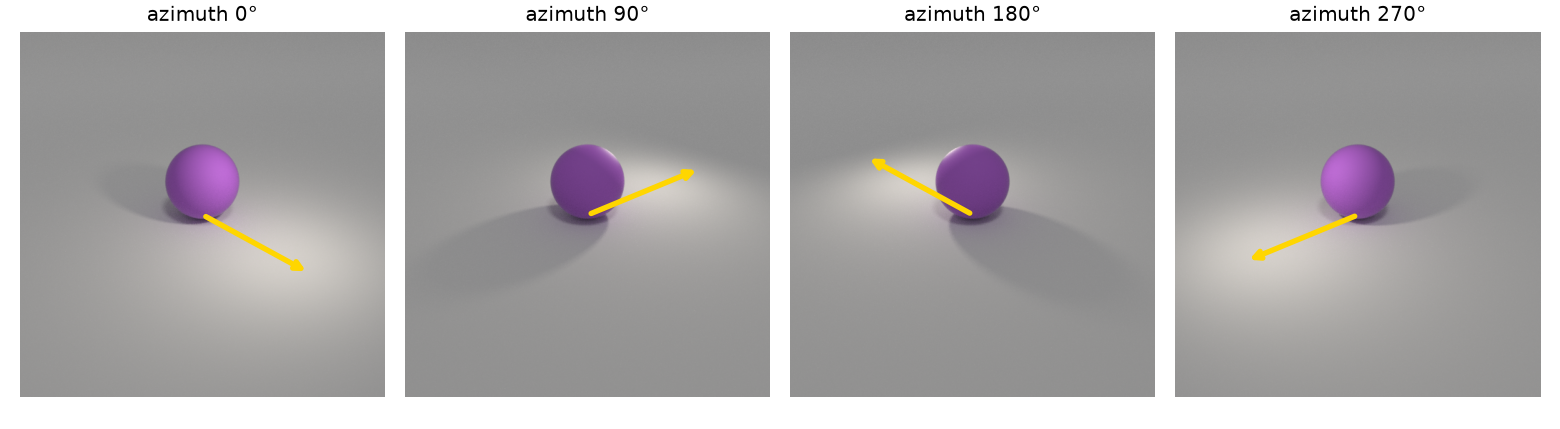
\includegraphics[width=\linewidth]{figures/conventions.png}
\caption{Renders with the key lamp at four azimuths ($\theta=45\degr$, sphere at the scene centre). The yellow line points to the lamp, as our geometry model predicts. The large floor highlight lies under the lamp and moves with the label.}
\label{fig:conventions}
\end{figure}

\paragraph{The label is the lamp position, not the light at the object.}
The lamp turns around the scene centre, but the object stands up to $2.8$ units from the centre.
The light direction at the object, $\mathrm{dir}(L-p)$ for lamp $L$ and object centre $p$, differs from the label by $35.0\degr$ in azimuth (mean) and by $16.2\degr$ in elevation.
The original probe follows the label: its azimuth MAE on cubes is $14.0\degr$ for the label and $35.5\degr$ for the light at the object.
So the probe reads the position of the lamp in the scene, and not the light that falls on the object.

\paragraph{Scene lights and a shortcut cue.}
The key lamp is an area lamp that always faces the scene centre.
It makes a bright spot on the floor between the lamp and the centre, and the position of this spot follows the label (Figure~\ref{fig:conventions}).
The spot is larger and brighter than the cast shadow, and it does not depend on the object shape.
The CLEVR base scene also contains a sun lamp that the modified script did not switch off. It gives $19\%$ of the floor brightness, as a constant front light.

\paragraph{A pitfall in the noise schedule.}
The original code noised the latent with \texttt{scheduler.add\_noise} of the SANA scheduler (\texttt{DPMSolverMultistepScheduler} with flow sigmas) before any call to \texttt{set\_timesteps}.
After construction, this scheduler stores variance-preserving sigmas in ascending order of the training step, while its timesteps are in descending order.
The function finds the index of $t$ in the descending list and reads the sigma of step $999-t$.
With flow sigmas it then computes $x_t=(1-\sigma)x_0+\sigma\epsilon$ with this value of $\sigma$.
Table~\ref{tab:noise} shows the result: for $t=200$ the transformer receives an input with $35$ times the expected norm and an inverted signal, while its timestep embedding says $\sigma=0.2$.
The stored activations agree: in block 4 the mean token norm is about $11{,}100$ at $t=200$ and $720$ at $t=800$.
The same order problem affects four schedulers of the library. We reported it to the maintainers, with a fix and tests (the link is withheld for anonymity).

\begin{table}[t]
\centering
\caption{Noise rule of the original code against the flow rule that SANA expects. Coefficients of the least-squares fit $x_t=a\,x_0+b\,\epsilon$.}
\label{tab:noise}
\begin{tabular}{rrrrr}
\toprule
$t$ & $a$ (original) & $b$ (original) & $a$ (flow) & $b$ (flow) \\
\midrule
200 & $-24.53$ & $25.53$ & $0.80$ & $0.20$ \\
500 & $-2.42$ & $3.42$ & $0.50$ & $0.50$ \\
800 & $0.28$ & $0.72$ & $0.20$ & $0.80$ \\
\bottomrule
\end{tabular}
\end{table}

\paragraph{Figures and probe fit.}
The figures of the original study drew the shadow direction with the default Blender camera and an orthographic projection (mean direction error $5.2\degr$), and about $18\%$ of the arrows ended outside the image.
The Ridge $\alpha$ had no effect (the same MAE for $\alpha$ from $10^{-3}$ to $10^{3}$), because the sums of squares of the PCA scores are many orders of magnitude larger.
The final configuration was selected with test data.

\section{Controls on the existing data}
\label{sec:controls}

All controls use the original splits and the same probe recipe (PCA with 256 components, then Ridge).
The PCA scores are centred, and the grid of $\alpha$ is relative to the sums of squares of the scores, so the penalty has an effect.
The validation split alone selects $\alpha$.
Intervals are 95\% bootstrap intervals over the test images (2000 samples).

\paragraph{Pixels.}
A probe on raw pixels is as good as the probe on SANA activations (Table~\ref{tab:original}): $11.8\degr$ against $13.0\degr$ on spheres and cylinders, and $14.3\degr$ against $14.0\degr$ on cubes.
The pixel grid that the validation split selects ($16\times16$) is better than SANA ($9.6\degr$ and $12.8\degr$).
The input image already contains the label in a linearly decodable form.

\paragraph{Image regions.}
To find the region that carries the information, we fit the probe on four variants of each image (Table~\ref{tab:cues}; Figure~\ref{fig:cues} in the appendix): the full image; the image with the object replaced by the floor colour; a crop of the object alone on a grey background; and only the position of the brightest floor region (two numbers).
The floor carries the label: without the object, the probe is better than with it ($9.4\degr$ against $14.3\degr$ on cubes).
The position of the floor highlight alone gives $17.6\degr$ on cubes.
The object alone predicts the light at the object well on known shapes ($7.7\degr$), but this cue does not transfer to cubes ($21.5\degr$) and it does not predict the lamp label ($44.3\degr$ on cubes).
Thus the transfer to cubes that the original study reported is a property of the floor cues, which do not depend on the object shape.

\begin{table}[t]
\centering
\caption{Pixel probes on image regions (test split: spheres and cylinders; cubes: \texttt{test\_cubes}). Global: the dataset label (lamp position). Local: the light direction at the object.}
\label{tab:cues}
\begin{tabular}{llrrrr}
\toprule
 & & \multicolumn{2}{c}{Test (spheres, cylinders)} & \multicolumn{2}{c}{Cubes} \\
Variant & Label & Azimuth & Elevation & Azimuth & Elevation \\
\midrule
full image & global & 11.8 [9.9, 14.2] & 5.6 & 14.3 [13.1, 15.5] & 6.2 \\
 & local & 11.3 [9.3, 13.3] & 8.8 & 11.6 [10.6, 12.7] & 7.7 \\
floor only & global & 7.9 [7.0, 9.0] & 3.9 & 9.4 [8.8, 10.0] & 4.3 \\
 & local & 13.5 [11.6, 15.5] & 7.3 & 12.3 [11.2, 13.4] & 7.2 \\
object only & global & 19.8 [17.5, 22.3] & 8.0 & 44.3 [41.9, 46.6] & 11.8 \\
 & local & 7.7 [6.8, 8.7] & 5.6 & 21.5 [20.3, 22.8] & 8.4 \\
highlight (2 numbers) & global & 12.2 [10.3, 14.5] & 7.4 & 17.6 [16.1, 19.3] & 8.1 \\
 & local & 30.4 [26.7, 34.5] & 13.8 & 30.7 [29.0, 32.4] & 14.1 \\
\bottomrule
\end{tabular}

\end{table}

\section{A corrected pipeline}
\label{sec:pipeline}

The corrected extraction (package \texttt{dd3d}) uses the flow rule $x_t=(1-t/1000)\,x_0+(t/1000)\,\epsilon$, a fixed noise seed for each image, and the attention mask of the empty prompt.
The features of all 20 blocks at $t\in\{100,200,400,600,800\}$ are average-pooled to a $4\times4$ grid, and blocks 4, 10 and 18 also to the $8\times8$ grid of the original study.
With the original noise rule, our extraction gives the token norms of the stored original activations, so the two pipelines differ only in the noise (Appendix~\ref{app:more}).

\paragraph{Controls.}
Each data set has the same probe on these inputs:
\begin{itemize}
    \item the input pixels at four grids ($8\times8$ to $64\times64$ px; the validation split selects the grid);
    \item the DC-AE latent;
    \item SANA-1.6B with random weights (the default initialization of the same architecture) \citep{adebayo2018sanity};
    \item the UNets of Stable Diffusion 1.5 and SDXL, with the noise rules of their own schedules;
    \item two vision encoders without a generative objective, DINOv2-L \citep{oquab2024dinov2} and CLIP ViT-L/14 \citep{radford2021clip} ($224$ px, no noise). They test whether the effect needs a generative model.
\end{itemize}

\paragraph{The original data with the corrected pipeline.}
We repeat the original experiment on the same images and splits (Table~\ref{tab:rq1}, rows v1).
With the original noise rule, the best SANA probe on the validation split gives $14.5\degr$ on cubes. This reproduces the original result and is $1.7\degr$ worse than the best pixel grid ($12.8\degr$).
With the flow rule, the best SANA probe (block~7, $t=100$) gives $4.8\degr$, $8.0\degr$ better than the pixels (95\% interval $[7.1, 8.9]$).
Thus the original study did not fail because SANA lacks the information: the wrong noise hid it.
The v1 images still have the floor highlight, so this result alone does not show a representation of the light at the object.

\section{Clean data: one directional light and a controlled position}
\label{sec:clean}

Table~\ref{tab:sets} lists the data sets. Each set has the splits of the original study.

\begin{table}[t]
\centering
\caption{Data sets. All sets except v1 use one sun lamp (a direction only) and a flat floor. The sets v2 to v2rot share the scenes (light, size, rotation of the object); v2r, v2rns and v2rso also share the positions.}
\label{tab:sets}
\begin{tabular}{lp{8.2cm}rl}
\toprule
Set & Change & Images & Use \\
\midrule
v1 & original data: area lamp around the scene centre, floor highlight, extra sun lamp & 3000 & audit \\
v2 & object at the scene centre & 3000 & probes, causal tests \\
v2ns & v2 without the cast shadow & 3000 & cue check \\
v2pos & v2 with the object at a random position (other scenes) & 300 & test of the v2 probes \\
v2r & v2 with the object at a random position & 3000 & main probe test \\
v2rns & v2r without the cast shadow & 3000 & cue variant \\
v2rso & v2r with the object hidden from the camera; its shadow stays & 3000 & cue variant \\
v2rot & 48 test scenes of v2 with the light azimuth $+90\degr$ & 48 & patch test \\
\bottomrule
\end{tabular}
\end{table}

\paragraph{Data set v2.}
We rendered 3000 new images with the same camera and object sizes, but with these changes: the key lamp is a sun lamp, so the label is exact at every point of the scene; the extra lamp is off; a flat floor replaces the curved backdrop; there is no camera jitter; and the object stands at the scene centre.

\paragraph{A centred object makes the pixel control almost perfect.}
On v2, the pixel probe has an azimuth MAE of $2.5\degr$ on spheres and cylinders and $13.7\degr$ on cubes.
With the object always at the same place, the shadow always falls in the same part of the image, and a linear read-out of the pixels needs no 3D knowledge.
The floor brightness also shows the elevation (floor alone: $1.7\degr$ on cubes), so we use the azimuth only.
The same pixel probe on v2pos (object at random positions) has $69.0\degr$, near the chance level of $90\degr$.

\paragraph{Data set v2r: a random position.}
Data set v2r has the same lights, sizes and rotations as v2, image for image; only the position changes.
The position is uniform on the part of $[-3,3]^2$ where the largest object is fully in the image, so it does not correlate with the light ($|r|\le0.02$).
On v2r, the pixel probe has $25.1\degr$ on spheres and cylinders and $25.8\degr$ on cubes; a pixel probe fitted on v2 has $71.2\degr$ and $70.4\degr$.
The information is still in the image: a crop of the object alone gives $4.4\degr$ on spheres and cylinders.
Thus a linear read-out of the pixels cannot find the light at an arbitrary place in the image, while a representation that does not depend on the position can.

\paragraph{Cue variants and weak cues.}
In v2rns the object casts no shadow, so only its shading is left; in v2rso the camera does not see the object, but its shadow stays.
A pair of images thus differs in one main cue only.
One weak cue stays in both variants: the purple object reflects light onto the floor on its lit side. Without the cast shadow (v2ns), the floor alone still gives $4.6\degr$.

\section{Probes on the clean data}
\label{sec:rq1}

\paragraph{Protocol.}
For each model we fit the probe on every block and on the timesteps $t\in\{100,200,400,600,800\}$ (DINOv2 and CLIP: every second layer, no noise).
The features of a block are the token means on a grid of $1\times1$, $2\times2$ or $4\times4$ cells, and also $8\times8$ cells for some blocks. The $1\times1$ grid has no information about the position.
The validation split selects the block, the timestep and the grid of each model.
The pixel baseline is the same probe on the RGB image at four resolutions, and the validation split also selects the resolution.
A coarse grid is often the stronger linear baseline, because it averages the position of the shadow.
A control task with shuffled train and validation labels gives a mean MAE of $82\degr$ to $98\degr$ for every source, so the probes do not fit noise \citep{hewitt2019control}.
Table~\ref{tab:rq1} compares each source with the best pixel grid on the same test images (paired bootstrap).

\begin{table}[t]
\centering
\caption{Azimuth MAE (degrees, 95\% interval) of the probe selected on the validation split. Test: spheres and cylinders; cubes: a shape that the probe did not see. Last column: paired difference to the best pixel grid on the cubes. Block names of the UNets follow the order down, mid, up; DINOv2 and CLIP get no noise ($t=0$).}
\label{tab:rq1}
\resizebox{\linewidth}{!}{\begin{tabular}{llllll}
\toprule
Data & Features & Block, $t$, grid & Test & Cubes & Cubes $-$ pixels \\
\midrule
v2r, no shadow & Pixels (best grid) & 16 px & $24.6$ \scriptsize{[20.7, 28.8]} & $23.3$ \scriptsize{[21.6, 24.9]} & -- \\
v2r, no shadow & DC-AE latent & -- & $29.0$ \scriptsize{[25.2, 33.0]} & $30.7$ \scriptsize{[29.0, 32.5]} & $+7.4$ \scriptsize{[+5.5, +9.6]} \\
v2r, no shadow & SANA-1.6B & 5, 100, 2 & $6.9$ \scriptsize{[6.2, 7.6]} & $9.9$ \scriptsize{[9.4, 10.4]} & $-13.4$ \scriptsize{[-14.9, -11.7]} \\
\midrule
v2r, only shadow & Pixels (best grid) & 8 px & $24.6$ \scriptsize{[20.7, 29.0]} & $16.9$ \scriptsize{[15.6, 18.1]} & -- \\
v2r, only shadow & DC-AE latent & -- & $15.7$ \scriptsize{[13.4, 18.2]} & $17.8$ \scriptsize{[16.5, 19.1]} & $+1.0$ \scriptsize{[-0.4, +2.4]} \\
v2r, only shadow & SANA-1.6B & 7, 100, 4 & $5.9$ \scriptsize{[5.2, 6.7]} & $7.9$ \scriptsize{[7.6, 8.3]} & $-8.9$ \scriptsize{[-10.2, -7.6]} \\
\bottomrule
\end{tabular}
}
\end{table}

\paragraph{With a random position, diffusion features are much better than a linear read-out of the input.}
On v2r the SANA probe (block 5, $t=100$, $2\times2$ grid) has an azimuth MAE of $5.4\degr$ on spheres and cylinders and $7.6\degr$ on cubes.
The best pixel grid gives $21.5\degr$ and $20.1\degr$, so SANA is better by $12.5\degr$ on cubes (95\% interval $[11.1, 13.8]$).
The DC-AE latent gives $18.8\degr$ and $19.0\degr$.
SD~1.5 ($7.5\degr$, $11.1\degr$) and SDXL ($5.9\degr$, $7.3\degr$) show the same effect.
SANA with random weights already beats the latent ($11.9\degr$, $15.9\degr$), so random nonlinear features help a linear probe; training halves the error.
Figure~\ref{fig:scan} shows that the best blocks are early and middle blocks (4 to 10) at the lowest noise level.

\paragraph{Models without a generative objective read the light equally well.}
DINOv2 and CLIP are better than SANA on spheres and cylinders on every data set, by $0.5\degr$ to $2.5\degr$ (paired intervals exclude zero); on v2r they give $3.3\degr$ and $3.9\degr$.
On cubes, SANA is clearly better only where the object moves and its shading is visible: on v2r by $2.4\degr$ against DINOv2 ($10.0\degr$) and by $8.4\degr$ against CLIP ($16.0\degr$), and on v2rns by $4.2\degr$ and $9.6\degr$.
On the other sets, also on v2rso where only the shadow is visible, the differences are below $1\degr$ in either direction.
A light direction that a linear probe can read is thus a property of good image features, not specific to a generative model.
Training for generation gives at most a code of the shading that transfers better to a new shape.
DINOv2 and CLIP get $224$~px images and SANA $1024$~px, so this comparison is not exact.

\begin{figure}[t]
\centering
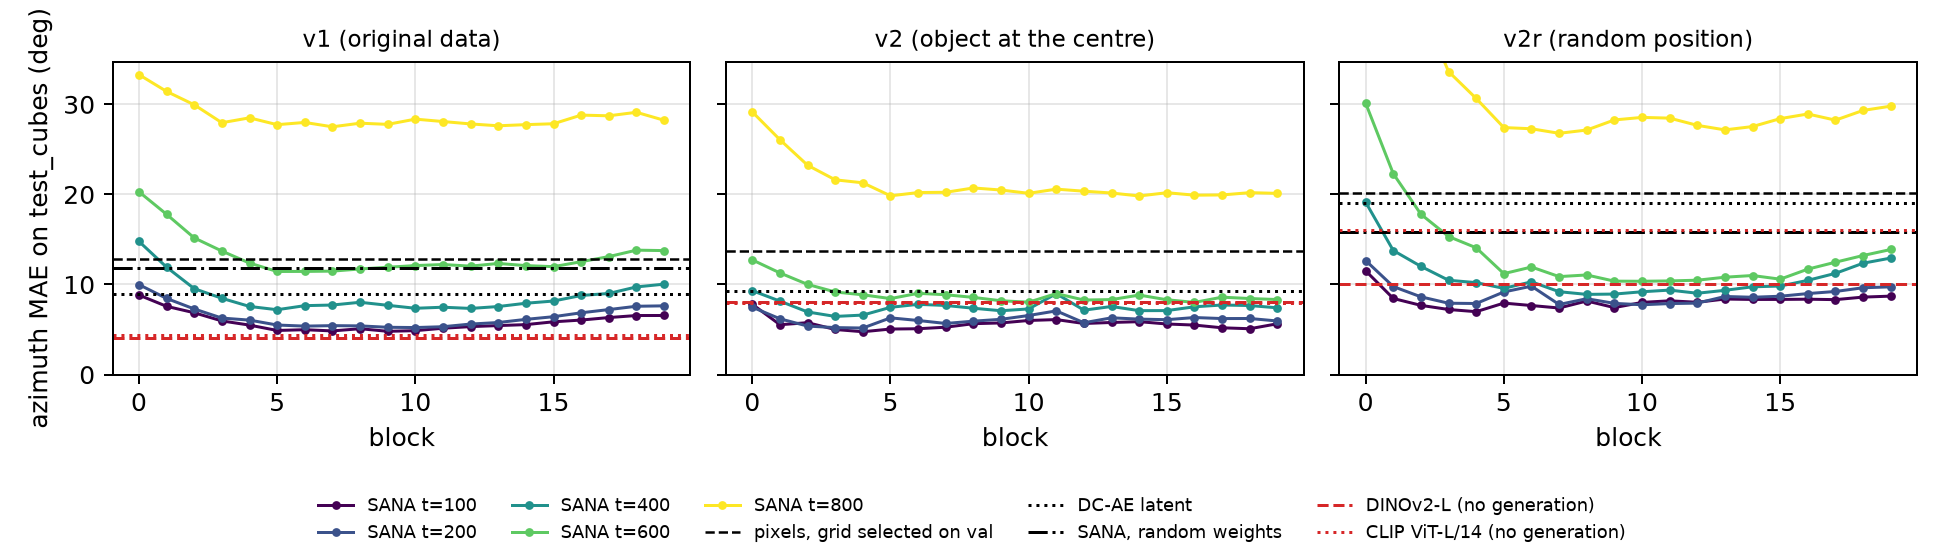
\includegraphics[width=\linewidth]{figures/scan.png}
\caption{Azimuth MAE on the cubes for the SANA probe on each block ($4\times4$ grid), one line for each timestep. Horizontal lines: the pixel grid that the validation split selects, the DC-AE latent, SANA with random weights, DINOv2 and CLIP, each at its setting from the validation split.}
\label{fig:scan}
\end{figure}

\paragraph{The representation depends little on the position.}
The mean of all tokens (the $1\times1$ grid) still gives $5.9\degr$ on spheres and cylinders of v2r ($13.2\degr$ on cubes).
A stronger test fits the probe on v2, where the object is always at the centre, and applies it to v2r.
The pixel probe fails ($71.2\degr$ and $70.4\degr$).
The SANA probe on the mean of all tokens gives $9.0\degr$ and $17.6\degr$; SD~1.5 gives $10.6\degr$ and $22.0\degr$, DINOv2 $6.8\degr$ and $21.5\degr$, and CLIP $8.0\degr$ and $19.0\degr$.
With the $8\times8$ grid, which keeps the position, the transfer is weaker (SANA: $38.4\degr$ and $40.9\degr$).
Thus each model has a direction code that is largely the same at every place in the image, and the cell features add a position-dependent part.
The transfer is not perfect: on cubes, the SANA probe from v2 is $4.4\degr$ worse than a probe fitted on v2r itself.

\paragraph{Both cues are readable.}
Without the cast shadow (v2rns), the SANA probe gives $6.9\degr$ and $9.9\degr$; the best pixel grid gives $24.6\degr$ and $23.3\degr$.
With only the shadow (v2rso), SANA gives $5.9\degr$ and $7.9\degr$, against $24.6\degr$ and $16.9\degr$ for the pixels.
So the model encodes the light without the cast shadow and also without the visible object, although both variants keep the weak floor cue.
A probe fitted on v2r partly transfers to the scenes with one cue ($33.3\degr$ without the shadow and $30.2\degr$ with only the shadow; pixels: $72.7\degr$ and $74.6\degr$), so the two cues share part of their code.
A map of the probe weights over the grid cells does not separate SANA from the pixels (Appendix~\ref{app:more}).

\section{Does the model use the direction?}
\label{sec:causal}

A probe shows that a property is readable, not that the model uses it \citep{elazar2021amnesic,belinkov2022probing}.
We test use with three interventions during generation.
All three start from a render of v2.
We encode the render, add flow noise up to $\sigma_0=0.7$, and integrate the flow back to $\sigma=0$ in 20 Euler steps \citep{meng2022sdedit}.
Without an intervention, this gives a close copy of the render (the base output).
A forward hook on one transformer block changes its output at every step.

\paragraph{Four measures of the output light.}
We compare each output with the base output of the same image and noise (Table~\ref{tab:measures}).
\begin{itemize}
    \item The \emph{pixel probe} ($64\times64$ pixels, fitted on the v2 renders) reads the azimuth from the whole image: the object, the cast shadow and the floor.
    \item The \emph{object probe} is the same probe on a crop of the object, with the floor set to grey. It reads the shading of the object alone.
    \item The \emph{dark-region measure} uses no fitted model. It takes the floor pixels that are more than 20 grey levels darker than the floor median, computes their darkness-weighted centroid, and turns the image vector from the object base to this centroid into a ground azimuth with the camera model. It fails on short shadows, so we report medians.
    \item The \emph{kept share} is the share of the crisp shadow pixels of the base output (40 grey levels below the floor median) that are still in shadow.
\end{itemize}
A centroid of dark pixels cannot separate a turned shadow from an old shadow plus a new dark region, so the kept share and a visual check complete it.
On renders, each measure sees a turn of the light by $90\degr$ (Table~\ref{tab:measures}).

\begin{table}[t]
\centering
\caption{The measures of the output light on renders with a known light. Error: median azimuth error on the v2 test renders (cubes in brackets). Turn: the median reading for a v2 render and the same scene with the light turned by $+90\degr$ (v2rot, 48 pairs).}
\label{tab:measures}
\begin{tabular}{lrr}
\toprule
Measure & Error & Turn of $+90\degr$ \\
\midrule
Pixel probe & $1.7\degr$ ($10.7\degr$) & $+90.7\degr$ \\
Object probe & $2.6\degr$ ($20.6\degr$) & $+89.1\degr$ \\
Dark region & $6.4\degr$ ($8.7\degr$) & $+83.5\degr$ \\
Kept share & -- & $0.07$ (same image: $1.00$) \\
\bottomrule
\end{tabular}
\end{table}

\paragraph{Shift along a direction.}
The probe of block $b$ is linear in the cell features: $\hat{\mathbf y}=W h+c$.
We add a vector $\delta$ to all tokens of each grid cell, which changes the cell mean by exactly $\delta$.
The \emph{probe direction} is the shortest change that turns the probe output by $90\degr$: $\delta=W^\top(WW^\top)^{-1}(R_{90}\hat{\mathbf y}-\hat{\mathbf y})$. We apply it as it is and scaled to the mean token norm of the block (r1).
A probe weight vector can contain directions that only cancel noise, so it is not the best candidate for a change that the model uses \citep{haufe2014interpretation,marks2024geometry}.
The \emph{activation pattern} comes from a least-squares regression of the features on $(\sin\phi,\cos\phi)$ over the train split, with the matrix $B$. Then $\delta=(\mathbf y(\phi+90\degr)-\mathbf y(\phi))B$ is the mean feature change between images whose light differs by $90\degr$. We apply it with factors 1 and 3.
Each family has a control: a random vector with, in each cell, the norm of the largest step of the family.
The plans use the features at $t=400$, inside the noise range of the test.
This is a form of activation steering \citep{turner2023activation,chen2023beyond}.

\paragraph{Erasure.}
LEACE \citep{belrose2023leace} removes the linear information about $(\sin\phi,\cos\phi)$ from features with the smallest change.
The \emph{pooled eraser} is one LEACE eraser for the cells of all positions. It removes only the part of the code that is the same in every cell: a new probe on the $8\times8$ grid still reads the azimuth after it ($4.7\degr$ against $4.6\degr$ in block~4).
The \emph{cell eraser} has one LEACE eraser for each grid cell. After it, a new probe on the grid is at chance ($88\degr$).
Its control fits the same cell erasers on the train labels in a random order, so it removes a subspace of the same rank but not the light code.
If the model uses the erased code in later blocks, the output light must change or become less consistent with the input light.

\paragraph{Patch test.}
The shift and the erasure depend on a linear direction; the patch test does not \citep{meng2022locating,zhang2024patching,basu2024localizing}.
For 48 test scenes of v2 we rendered a second image of the same scene with the light azimuth $+90\degr$ (set v2rot).
Both images get the same noise.
The source pass (v2rot) records the output of a block at every step, and in the target pass (v2) the tokens of one region get the recorded values.
The regions come from the scene geometry: all tokens, the object, the cast shadow of the source light, and the rest of the floor.
A patched token copies the source image at its own place, and the object cells also hold the floor next to the object, where the shadow starts.
Thus we also measure the source shadow outside the patched cells, grown by one token (16~px). Only this part shows a shadow that the model draws at another place.

\paragraph{Results of the shift.}
Table~\ref{tab:causal} gives the results for 60 test images of v2 and three blocks.
The probes come from the $8\times8$ features at $t=400$ (test MAE $4.4\degr$ to $4.6\degr$).
The base output keeps the light of the render (pixel probe MAE $7.6\degr$ against the label).
A random change of the base output keeps $82\%$ to $88\%$ of its crisp shadow, so this is the level of no effect.
\begin{itemize}
    \item The pattern direction at the natural size ($\times1$) turns the object probe by $+50\degr$ to $+52\degr$ and the pixel probe by $+60\degr$ to $+65\degr$, towards the target of $+90\degr$. The change has a mean cell norm of $2\%$ of the token norm, and the image changes by $4$ grey levels. The crisp shadow stays ($68\%$ to $80\%$ kept), and the dark region turns by only $+5\degr$ to $+7\degr$. The shift changes the shading of the object, not the cast shadow.
    \item With $\times3$ the object probe turns by $+71\degr$ to $+82\degr$. Only $32\%$ to $40\%$ of the old crisp shadow stays, and a diffuse dark region appears on the floor towards the target, which turns the dark-region measure by $+92\degr$ to $+109\degr$. The images show no new crisp shadow (Figure~\ref{fig:causal_examples}).
    \item A random vector with the same norm in each cell does nothing.
    \item The shortest change along the probe weights turns the object probe by only $+22\degr$ to $+29\degr$. At the size of the token norm, it destroys the image in blocks 4 and 10 (mean change above 100 grey levels). In block 18 it turns the pixel probe by $+84\degr$ but the object probe by only $+11\degr$: the whole-image reading then comes from changes of the floor.
\end{itemize}
Thus the pattern direction is a causal handle on the shading of the object. The probe weights are a worse handle, as \citet{haufe2014interpretation} predict for a regression with correlated noise.
The same holds for the pattern of block~5 at $t=100$, the best probe on v2r, with a clear dose effect; with more noise ($\sigma_0=0.85$ and $0.95$) the base output loses the input light and the effects become small (Appendix~\ref{app:more}, Table~\ref{tab:causal_more}).
A shift of the pattern in all 20 blocks at the same time turns all measures, but it draws dark and bright blocks on the grid of the shift, not a new shadow (Figure~\ref{fig:multi}).
None of our shifts drew a new crisp shadow. A shift that is constant in each cell cannot draw a sharp shape by itself, so this result concerns such shifts only.

\begin{table}[t]
\centering
\caption{Shift test: output light against the base output for a target of $+90\degr$, 60 images of v2. Each cell gives blocks 4 / 10 / 18. Probes: mean rotation (degrees); dark region: median rotation; kept share of the crisp shadow; pixels: mean absolute change (grey levels). The rows \texttt{probe\_r1} and \texttt{random\_probe} destroy the image in blocks 4 and 10, so their readings there have no meaning.}
\label{tab:causal}
\resizebox{\linewidth}{!}{\begin{tabular}{lrrrrrrr}
\toprule
 & \multicolumn{2}{c}{Block 4} & \multicolumn{2}{c}{Block 10} & \multicolumn{2}{c}{Block 18} & \\
Condition & probe & shadow & probe & shadow & probe & shadow & pixels \\
\midrule
probe\_exact & $+41$ \scriptsize{[+36, +46]} & $+4$ & $+23$ \scriptsize{[+20, +26]} & $+1$ & $+40$ \scriptsize{[+36, +44]} & $+2$ & 2 \\
probe\_r1 & $-4$ \scriptsize{[-30, +21]} & $+83$ & $-3$ \scriptsize{[-28, +21]} & $+81$ & $+84$ \scriptsize{[+80, +89]} & $+46$ & 107 \\
random\_probe & $-3$ \scriptsize{[-26, +20]} & $-22$ & $-5$ \scriptsize{[-31, +21]} & -- & $+14$ \scriptsize{[-3, +32]} & $-3$ & 138 \\
pattern\_x1 & $+65$ \scriptsize{[+60, +71]} & $+7$ & $+60$ \scriptsize{[+55, +65]} & $+7$ & $+62$ \scriptsize{[+58, +68]} & $+5$ & 4 \\
pattern\_x3 & $+121$ \scriptsize{[+117, +125]} & $+109$ & $+121$ \scriptsize{[+116, +125]} & $+107$ & $+120$ \scriptsize{[+115, +124]} & $+92$ & 13 \\
random\_pattern & $0$ \scriptsize{[-1, +1]} & $0$ & $0$ \scriptsize{[-3, +2]} & $-1$ & $-2$ \scriptsize{[-5, +1]} & $0$ & 2 \\
erase & $0$ \scriptsize{[-1, 0]} & $0$ & $0$ \scriptsize{[-1, 0]} & $0$ & $0$ \scriptsize{[-1, +1]} & $0$ & 2 \\
\bottomrule
\end{tabular}
}
\end{table}

\begin{figure}[t]
\centering
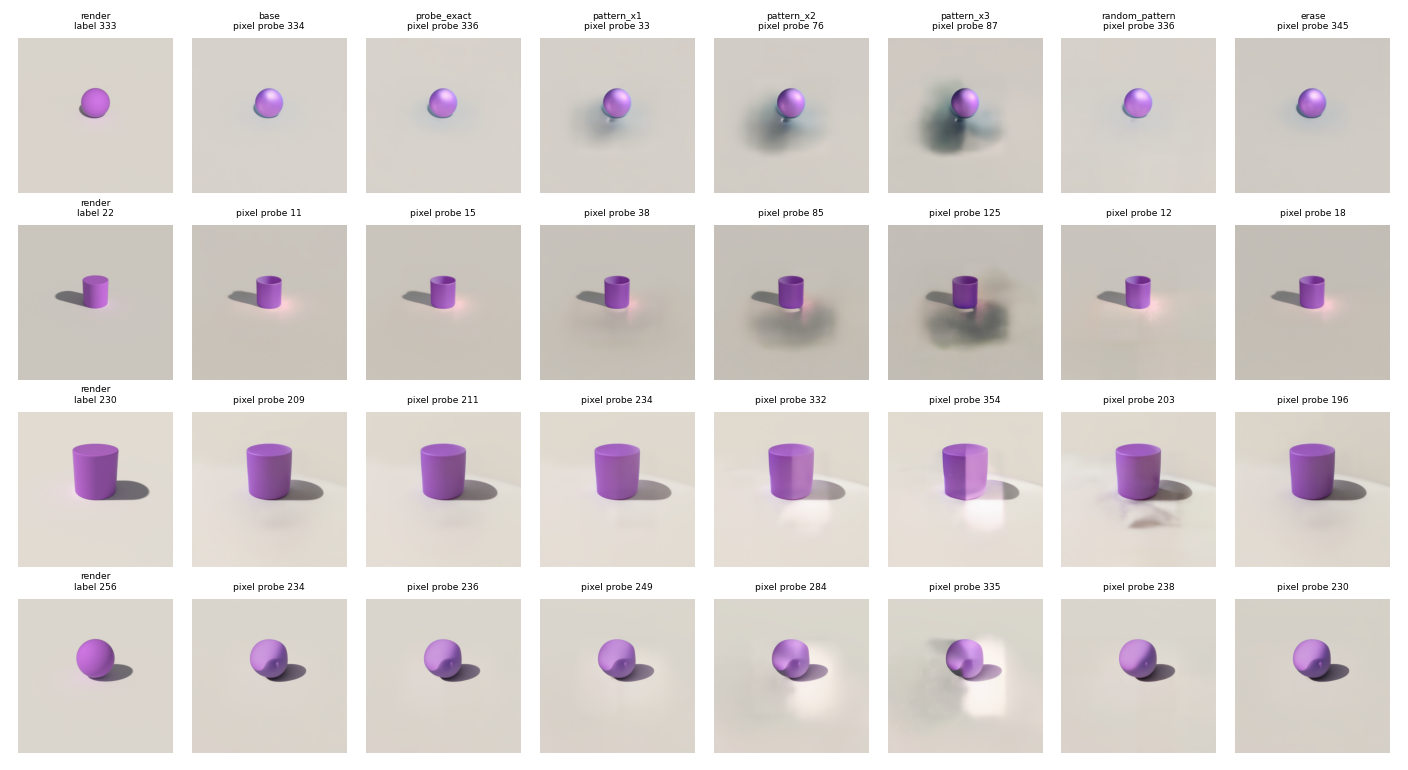
\includegraphics[width=\linewidth]{figures/causal_examples.png}
\caption{Four test images: the render, the base output and each condition of the shift test in block~5 ($t=100$ pattern). Large pattern steps darken the floor towards the target, but the crisp shadow keeps its place. Titles: the azimuth that the pixel probe reads.}
\label{fig:causal_examples}
\end{figure}

\paragraph{Results of the erasure.}
The pooled eraser has no effect on any measure (rotation $0\degr$, kept share $0.93$ to $0.99$), as expected from an eraser that leaves the code in the cells.
Table~\ref{tab:erase} in Appendix~\ref{app:more} gives the cell eraser and its control.
In blocks 4, 10 and 18 at $t=400$, the cell eraser increases the azimuth error of the output from $7.6\degr$ to $21.9\degr$, $30.4\degr$ and $44.2\degr$; its control gives $8.7\degr$ to $9.6\degr$.
The mean rotation stays near $0\degr$, so the light does not turn to one side: it agrees less with the input.
The crisp shadow of the base output also stays less often (kept share $0.65$ to $0.79$, control $0.92$ to $0.95$).
Two facts limit this result.
The control changes the features about three times less ($0.4\%$ to $0.7\%$ of the token norm, against $1.2\%$ to $1.8\%$), because shuffled labels give only a weak linear relation.
And the cell eraser adds local grey smears near the object (Figure~\ref{fig:erase_examples}).
In block~5 at $t=100$, the control also breaks the output (error $31.1\degr$), so this setting cannot separate the two erasers.


\paragraph{Results of the patch test.}
Figure~\ref{fig:patch} gives the results for 48 pairs.
The full source pass turns the pixel probe by $1.01$ of the $90\degr$ offset and the object probe by $0.56$; the object probe reads generated images less well than renders.
A patch of all tokens of block~10 moves $0.73$ of the pixel-probe rotation and $84\%$ of the crisp source shadow.
A patch of the object tokens (about $10\%$ of the image) moves $0.57$ to $0.63$ of the pixel-probe rotation and $0.36$ to $0.45$ of the object-probe rotation in every block from 0 to 18, about three quarters of the full source pass.
In the whole image, $33\%$ to $38\%$ of the source shadow appears, but this is mostly a copy: on average $42\%$ of the source shadow lies in the object cells.
Outside these cells, $3\%$ to $9\%$ of the source shadow appears, against $3\%$ without a patch, and $79\%$ to $97\%$ of the target shadow stays. The small gain is mostly in blocks 0 to 8.
A patch of the source-shadow tokens copies the source shadow to its place but keeps the target shadow: the output has two shadows.
Thus the object tokens carry the light code that sets the shading of the object, but not the cast shadow.
The shadow comes from the tokens at its own place, and only a patch of all tokens moves it.
The results are the same in every block, because a patch of a token replaces its whole state, which later blocks only refine.

\begin{figure}[t]
\centering
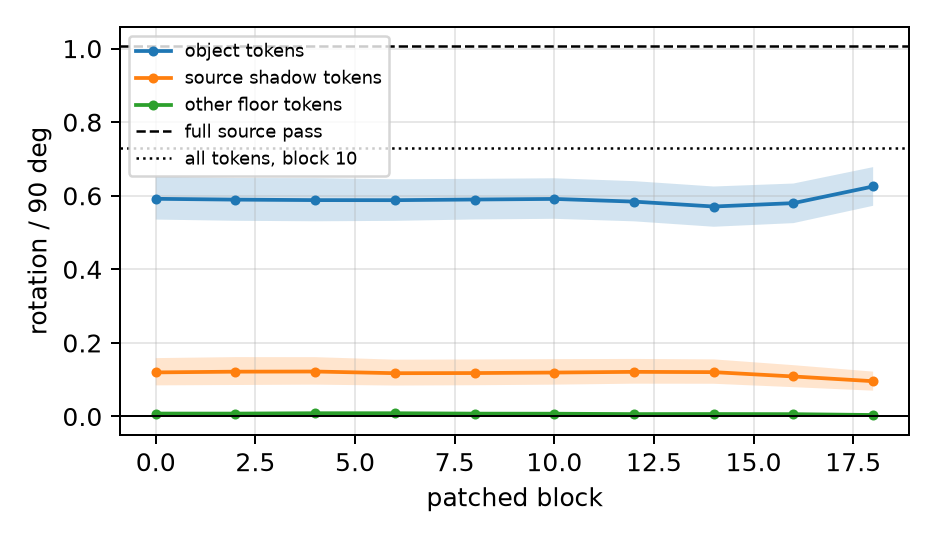
\includegraphics[width=\linewidth]{figures/patch.png}
\caption{Patch of one region in one block, 48 pairs (source light $+90\degr$). Left and middle: share of the rotation that the pixel probe and the object probe read. Right: the share of the crisp source shadow that appears outside the patched cells (grown by 16~px), minus the same share without a patch. Lines: the full source pass and a patch of all tokens in block~10.}
\label{fig:patch}
\end{figure}

\section{Discussion}
\label{sec:discussion}

\paragraph{What the original result shows.}
The original probe reads the lamp position, and pixels give the same accuracy because a floor highlight follows the label.
The result therefore does not show that SANA represents the light direction.
It also does not show the opposite: with the flow noise, the same probe on the same data is much better than the pixels.
The noise pitfall hid the information; the shortcut made the pixels look as good as the model.

\paragraph{What the new results show.}
On scenes where the object moves, a linear probe on the pixels cannot find the light, and a linear probe on the activations of three diffusion models can.
The code depends little on the position, and the model reads the light from the shading and from the cast shadow, each one alone.
But this is not evidence of a generative world model. Two encoders without a generative objective read the light equally well, and a network with random weights already beats the pixels.
SANA uses its code for the shading of the object: a shift along the activation pattern turns it, a random shift does not, and the object tokens carry it.
We found no link between this code and the cast shadow, which needs the 3D relation between light, object and floor.
Our shifts do not draw a new shadow, and the object tokens do not move the shadow outside their own cells.
The cell eraser suggests that later blocks need the code: without it, the output light agrees less with the input. This effect is larger than the effect of the control eraser, but the control changes the features less, so the evidence is not final.
The data do not show if the model uses a second code for the shadow that our linear and local handles do not reach.

\paragraph{Probes and their measures.}
Three results warn against simple measures.
The probe weights are a poor steering handle, while the activation pattern works \citep{haufe2014interpretation}.
A measure that reads the whole image can report a large rotation when only the floor or the shading changes.
And a patch can look like a transfer of the shadow when it only copies the pixels of the patched tokens.
A claim that a model ``moves the shadow'' needs a measure of the shadow outside the changed region.

\paragraph{A checklist for probe studies of generative models.}
\begin{enumerate}
    \item Compare every probe with the same probe on the input pixels (at several resolutions), on the latent of the autoencoder, and on strong image encoders without a generative objective.
    \item Compare with the same architecture with random weights.
    \item Check the noise that the model receives: fit $x_t=a\,x_0+b\,\epsilon$ and compare with the schedule of the model.
    \item Define the label at the place of the effect, and store all scene parameters (camera, all lamps).
    \item Remove or randomize shortcut cues, vary the object position, and separate the cues with paired renders.
    \item Select the layer, the timestep and all hyperparameters on validation data only, and report intervals and paired comparisons.
    \item Test causal use. Steer along the activation pattern, not only along the probe weights, and compare with a random change of the same size. Fit an eraser for each position if the code depends on the position, and compare it with a control eraser.
    \item Measure the effect of an intervention with several independent measures, one of them specific to the cue in question and outside the changed region.
    \item Check figures against the true geometry.
\end{enumerate}

\section{Limitations}
The study uses one property, simple synthetic scenes with one object, and the empty prompt.
All interventions start from a render (SDEdit); at $\sigma_0=0.7$ the noisy input still shows the original shadow, which can resist a change.
Most interventions act in one block at a time, and all shifts are constant in each grid cell.
The object probe has larger errors on generated images than on renders, and the dark-region measure has large errors on short shadows.
The causal tests use 60 images (48 for the shift in all blocks), and the patch test uses 48 pairs.
The features are average-pooled, so the probes cannot see fine structure inside a cell.
DINOv2 and CLIP get smaller images than SANA.

\section{Conclusion}
A probe that reads a scene property from a generative model is a starting point, not evidence of 3D knowledge.
In the case that we studied, the first probe result was right for the wrong reasons. The shortcut made the pixels as good as the model, and a noise pitfall made the model look no better than the pixels.
With correct noise, controlled data and controls, SANA carries the light direction in a form that the input pixels do not offer, but so do image encoders that never generate images.
SANA uses this code to light the object. We found no evidence that it uses the same code to draw the cast shadow.
We release the tools so that other studies can run the same checks.

\paragraph{Reproducibility.}
The code, the job specifications, the result tables and the unit tests are in the supplementary material.
Every number in this paper comes from a script in the repository. The GPU and CPU jobs ran on Kaggle, and their specifications record the commit of each run.

\bibliography{references}
\bibliographystyle{tmlr}

\appendix
\section{Geometry of the renders}
\label{app:geometry}
The camera position is $c=c_0+j$ with $c_0=(7.481,-6.508,5.344)$ and jitter $j\in[-0.5,0.5]^3$.
The view direction is $f=-c/\lVert c\rVert$, the right axis is $r=f\times e_z/\lVert f\times e_z\rVert$ and the up axis is $u=r\times f$.
For a point $p$, let $d=p-c$; the pixel position is $x=W\,(0.5+\tfrac{35}{32}\,\tfrac{d\cdot r}{d\cdot f})$ and $y=H-H\,(0.5+\tfrac{35}{32}\,\tfrac{d\cdot u}{d\cdot f})$ with $W=H=512$.
The key lamp is at $L=5(\cos\theta\cos\phi,\cos\theta\sin\phi,\sin\theta)$.
The shadow of the object centre $p$ on the floor is $L+\tfrac{L_z}{L_z-p_z}(p-L)$.
For the sun lamp of the new data sets with the light direction $u$ (unit vector to the light), the shadow of a point $p$ is $p-\tfrac{p_z}{u_z}\,u$.
Renders without the object confirm the shadow arrows of this model: for scenes with long shadows, the mean angle between our arrow and the measured shadow is $4.7\degr$ ($7.6\degr$ for the original arrows).

\section{Experimental details}
\label{app:details}

\paragraph{Renders.}
Blender 2.78c with Cycles renders each image with 64 samples at $512\times512$ px.
The sets v2 to v2rot have a sun lamp with strength $3.0$ and a soft size of $0.02$, a white world light of strength $0.2$, a flat floor and no camera jitter. The extra lamp of the CLEVR scene is off.
The elevation is $\mathcal{U}(30\degr,75\degr)$, the object size $r$ is uniform in $[0.8,1.4]$ and its rotation is uniform in $[0,2\pi)$.
In v2rns the object casts no shadow (Cycles shadow visibility off); in v2rso the camera does not see the object (camera visibility off). In both sets the object still reflects light.

\paragraph{Features.}
SANA-1.6B runs in float16 on a T4 GPU with a $1024\times1024$ input (bilinear scale), the empty prompt with its attention mask, and the flow noise with a fixed seed for each image.
SANA with random weights uses the default initialization of the architecture.
Stable Diffusion 1.5 uses $512$ px and SDXL $1024$ px; their VAE runs in float32 and their UNet in float16, with the DDPM noise of each model. The blocks are the outputs of the down, mid and up blocks.
DINOv2-L and CLIP ViT-L/14 get the image at $224$ px without a crop, with the normalization of each model. Their features are the patch tokens of every second layer, without the class token.

\paragraph{Probe.}
A randomized PCA (at most 256 components) and the Ridge regression are fitted on the train split. The grid of $\alpha$ has 19 values from $10^{-5}$ to $10$ times the median sum of squares of the scores. The validation split selects $\alpha$, and the block, timestep and grid of each model, by the sum of the azimuth and elevation MAE.
The intervals are percentile intervals of 2000 bootstrap samples over the images; a paired comparison uses the same samples for both sources.

\paragraph{Causal tests.}
The tests use 60 test images of v2 (a random sample with a fixed seed), $\sigma_0=0.7$ unless stated, and 20 Euler steps $x_{\sigma'}=x_\sigma+(\sigma'-\sigma)\,v_\theta(x_\sigma,\sigma)$; the transformer gets the timestep $1000\,\sigma$.
A hook changes the output of one block at every step. The decoder output ($1024$ px) is scaled to $512$ px for the measures.
The pooled eraser is one LEACE eraser, fitted on 30{,}000 cells of the train images. The cell eraser has one LEACE eraser for each grid cell, fitted on all train images.

\paragraph{Patch test.}
The regions come from the scene geometry on a $16\times16$ grid. A cylinder with radius $r$ and height $2r$ stands for the object, and its shadow comes from the sun direction.
The object region has the cells that contain the object; the shadow region has the cells that contain the shadow but not the object.

\section{More results}
\label{app:more}

\paragraph{Agreement with the original pipeline and numeric precision.}
With the original noise rule, our extraction gives a mean token norm of $11{,}147$ in block~4 at $t=200$; the stored original activations have about $11{,}100$. With the flow rule, the norm is $718$.
On the same 12 images, float16 and float32 give the same features (relative difference $0.1\%$). The original noise rule overflows in float16 in block 18, so this control runs in float32.

\paragraph{Image regions of the original data.}
Figure~\ref{fig:cues} shows the image variants of Table~\ref{tab:cues}.

\begin{figure}[h]
\centering
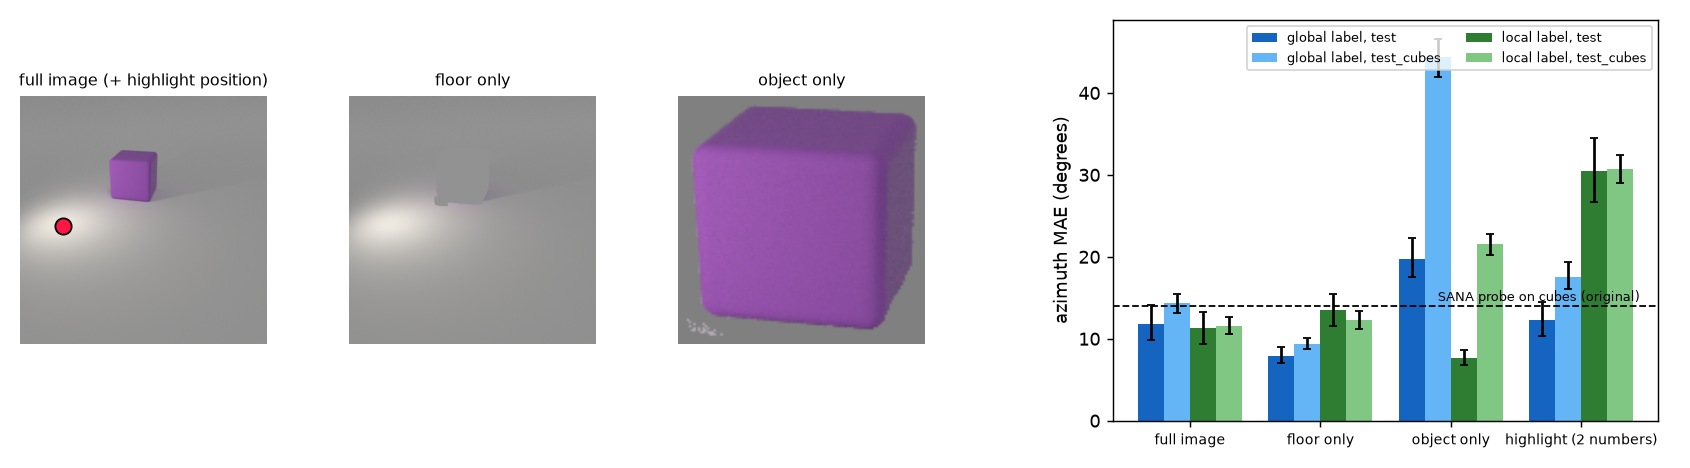
\includegraphics[width=\linewidth]{figures/cues.png}
\caption{Left: the image variants for the region probes (the red dot marks the floor highlight). Right: azimuth MAE with 95\% intervals. The dashed line is the original SANA probe on cubes.}
\label{fig:cues}
\end{figure}

\paragraph{Where the probe reads.}
The exact decomposition of a linear probe over the grid cells gives the share of each cell in the output (Figure~\ref{fig:maps}).
On v1 the pixel probe spreads its weight over the floor, where the highlight moves; on v2 it lies around the object and its shadow.
On v2r the SANA probe (block~10, $t=100$, $8\times8$) gives $20\%$ of its weight to the object cells and $5.4\%$ to the shadow cells, whose area shares are $14.5\%$ and $3.7\%$. The pixel probe on an $8\times8$ grid has almost the same shares ($19.6\%$ and $5.3\%$), so the maps do not separate the models.

\begin{figure}[h]
\centering
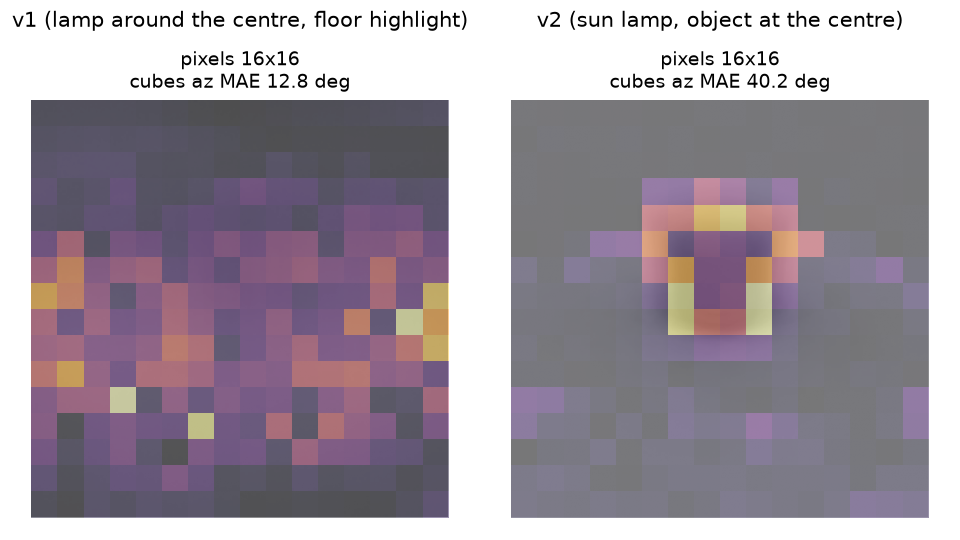
\includegraphics[width=0.7\linewidth]{figures/probe_maps_pixels.png}
\caption{Exact spatial decomposition of a linear probe on $16\times16$ pixels (brighter cells have a larger share of the azimuth output) on the original data (left) and on v2 (right). The title of each map gives the error of this $16\times16$ probe on cubes; Table~\ref{tab:rq1} uses the grid that the validation split selects.}
\label{fig:maps}
\end{figure}

\paragraph{Other shift tests.}
Table~\ref{tab:causal_more} gives the shift test with the pattern of block~5 at $t=100$ ($4\times4$ grid, test MAE $2.6\degr$), the best probe on v2r. The effect grows with the dose; at $\times2$ the shading reaches the target in all 60 images, while half of the old shadow stays.
With more noise, the base output keeps less of the input light (MAE $34.8\degr$ at $\sigma_0=0.85$ and $70\degr$ at $0.95$). At $\sigma_0=0.85$ the pattern ($\times1$) still turns the pixel probe by $+63\degr$, but the dark region does not turn, so the weak response of the shadow is not an effect of the input alone.
Figure~\ref{fig:multi} shows the shift of the pattern in all 20 blocks at the same time ($t=100$ features, 48 images). A quarter of the natural size turns the pixel probe by $+120\degr$, the object probe by $+81\degr$ and the dark region by $+107\degr$, and $37\%$ of the old shadow stays; the images change by 20 grey levels.

\begin{table}[h]
\centering
\caption{More shift tests. Rotation of the pixel probe and the object probe (mean) and of the dark region (median) in degrees, kept share of the crisp shadow, mean pixel change. Target: $+90\degr$; 60 images of v2 (48 for all blocks). At $\sigma_0=0.85$ and $0.95$ the base output has lost much of the input light, so the object probe is unreliable there.}
\label{tab:causal_more}
\begin{tabular}{llrrrrr}
\toprule
Setting & Condition & Pixel probe & Object probe & Dark region & Kept & Pixels \\
\midrule
Block 5, $t=100$ & pattern $\times1$ & $+30$ & $+20$ & $+2$ & $0.76$ & 4 \\
 & pattern $\times2$ & $+79$ & $+48$ & $+40$ & $0.55$ & 9 \\
 & pattern $\times3$ & $+105$ & $+69$ & $+88$ & $0.41$ & 13 \\
 & random & $+1$ & $-1$ & $0$ & $0.88$ & 1 \\
\midrule
Block 4, $\sigma_0=0.85$ & pattern $\times1$ & $+63$ & $+37$ & $-9$ & $0.49$ & 8 \\
 & pattern $\times3$ & $+92$ & $+7$ & $-3$ & $0.40$ & 20 \\
 & random & $+1$ & $+22$ & $0$ & $0.73$ & 2 \\
\midrule
Block 4, $\sigma_0=0.95$ & pattern $\times1$ & $+27$ & $-4$ & $+2$ & $0.67$ & 12 \\
 & random & $+7$ & $-1$ & $+2$ & $0.78$ & 4 \\
\midrule
All 20 blocks, $t=100$ & pattern $\times0.25$ & $+120$ & $+81$ & $+107$ & $0.37$ & 20 \\
 & pattern $\times0.5$ & $+129$ & $+71$ & $+129$ & $0.31$ & 32 \\
 & pattern $\times1$ & $+124$ & $+40$ & $+132$ & $0.26$ & 47 \\
 & random & $0$ & $+1$ & $0$ & $0.85$ & 4 \\
\bottomrule
\end{tabular}
\end{table}

\begin{figure}[h]
\centering
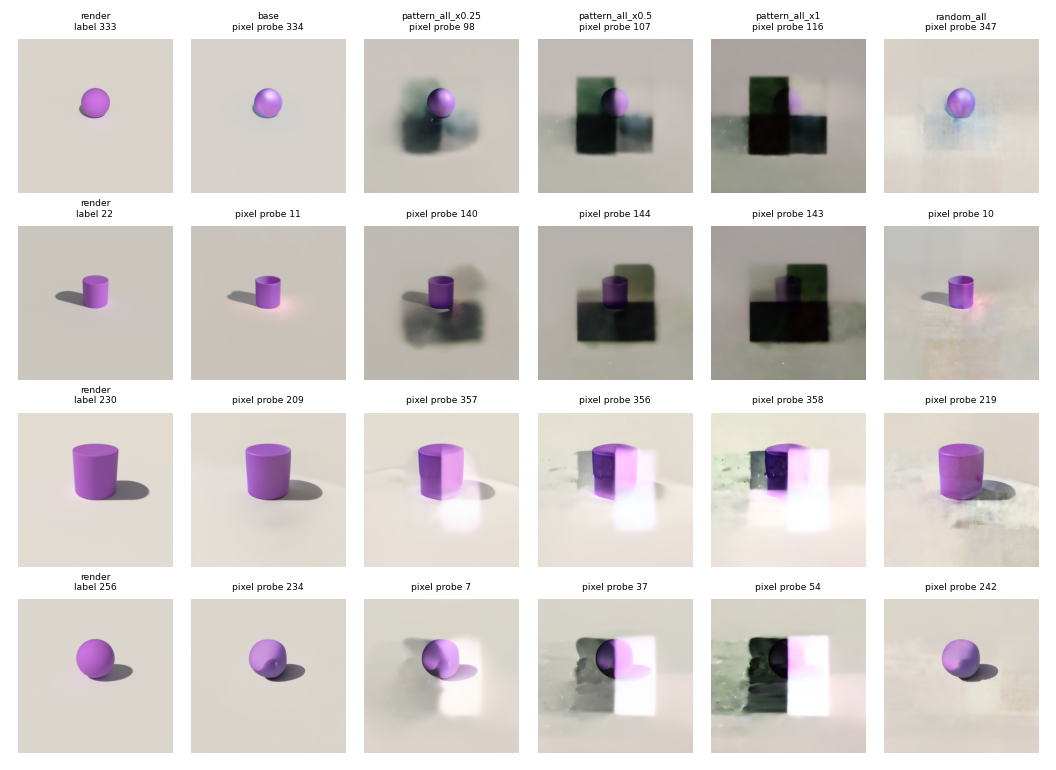
\includegraphics[width=\linewidth]{figures/causal_multi_examples.png}
\caption{Shift of the pattern in all 20 blocks at the same time ($t=100$ features, $4\times4$ grid). The shading of the object turns, but the floor shows dark and bright blocks on the grid of the shift, not a new cast shadow. A random shift of the same size (last column) has no effect.}
\label{fig:multi}
\end{figure}

\begin{table}[h]
\centering
\caption{Erasure test, 60 images of v2. Features: the azimuth MAE of a new probe on the $8\times8$ grid after the eraser (test split), and the mean change of a cell as a percentage of the token norm. Output: azimuth error of the pixel probe against the input label, median absolute rotation of the dark region (degrees), kept share of the crisp shadow, and mean pixel change (grey levels). The control eraser is fitted on shuffled labels.}
\label{tab:erase}
\resizebox{\linewidth}{!}{\begin{tabular}{llrrrrrr}
\toprule
 & & \multicolumn{2}{c}{Features} & \multicolumn{4}{c}{Output} \\
Block & Eraser & Probe & Change (\%) & Error & $|$Turn$|$ & Kept & Pixels \\
\midrule
4, $t=400$ & none & $4.6$ & -- & $7.6$ & $0$ & $1.00$ & $0$ \\
 & pooled & $4.7$ & -- & $7.7$ & $1$ & $0.98$ & $1.8$ \\
 & cell & $88.3$ & $1.2$ & $21.9$ & $12$ & $0.79$ & $2.9$ \\
 & cell, control & $4.9$ & $0.4$ & $8.7$ & $3$ & $0.93$ & $1.2$ \\
\midrule
10, $t=400$ & none & $4.4$ & -- & $7.6$ & $0$ & $1.00$ & $0$ \\
 & pooled & $4.5$ & -- & $7.9$ & $1$ & $0.99$ & $1.5$ \\
 & cell & $88.3$ & $1.3$ & $30.4$ & $13$ & $0.73$ & $2.6$ \\
 & cell, control & $4.5$ & $0.4$ & $9.2$ & $3$ & $0.95$ & $1.1$ \\
\midrule
18, $t=400$ & none & $4.5$ & -- & $7.6$ & $0$ & $1.00$ & $0$ \\
 & pooled & $4.3$ & -- & $7.8$ & $3$ & $0.93$ & $2.1$ \\
 & cell & $88.3$ & $1.8$ & $44.2$ & $32$ & $0.65$ & $2.9$ \\
 & cell, control & $4.5$ & $0.7$ & $9.6$ & $3$ & $0.92$ & $1.9$ \\
\midrule
5, $t=100$ & none & $2.6$ & -- & $7.6$ & $0$ & $1.00$ & $0$ \\
 & pooled & $2.9$ & -- & $11.1$ & $6$ & $0.99$ & $4.0$ \\
 & cell & $88.3$ & $1.5$ & $42.5$ & $35$ & $0.60$ & $5.1$ \\
 & cell, control & $2.8$ & $0.3$ & $31.1$ & $26$ & $0.71$ & $10.8$ \\
\bottomrule
\end{tabular}
}
\end{table}

\begin{figure}[h]
\centering
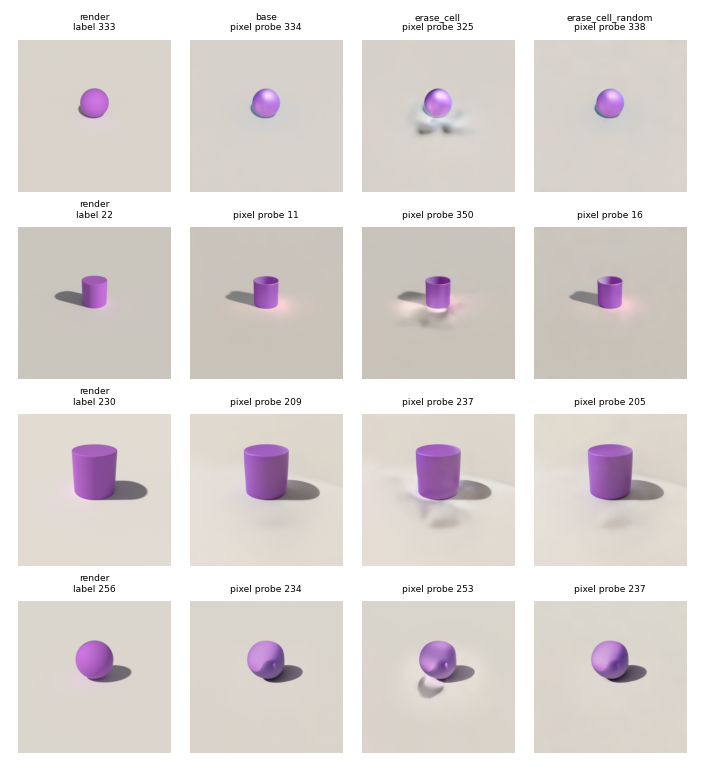
\includegraphics[width=0.7\linewidth]{figures/erase_examples.png}
\caption{Erasure in block~10 ($t=400$). Columns: the render, the base output, the cell eraser and its control. After the cell eraser, the crisp shadow often stays, but grey smears appear near the object. The control eraser keeps the image. Titles: the azimuth that the pixel probe reads.}
\label{fig:erase_examples}
\end{figure}

\end{document}
